\documentclass{standalone}
\usepackage{tikz}
\usepackage{pgfplots}
\pgfplotsset{compat=newest}
\usepackage{amsmath}
\usepackage[american]{circuitikz}
\usepackage{cmbright}

\definecolor{myred}{RGB}{170,0,0}
\definecolor{myblue}{RGB}{0,0,220}
\definecolor{mygreen}{RGB}{0,150,0}
\definecolor{myorange}{RGB}{255,127,0}
\definecolor{mybrown}{RGB}{150,75,0}

\ctikzset{bipoles/resistor/height=0.2}
\ctikzset{bipoles/resistor/width=0.5}
\ctikzset{bipoles/capacitor/height=0.4}
\ctikzset{bipoles/capacitor/width=0.15}
\ctikzset{bipoles/diode/height=0.5}
\ctikzset{bipoles/diode/width=0.4}

\begin{document}
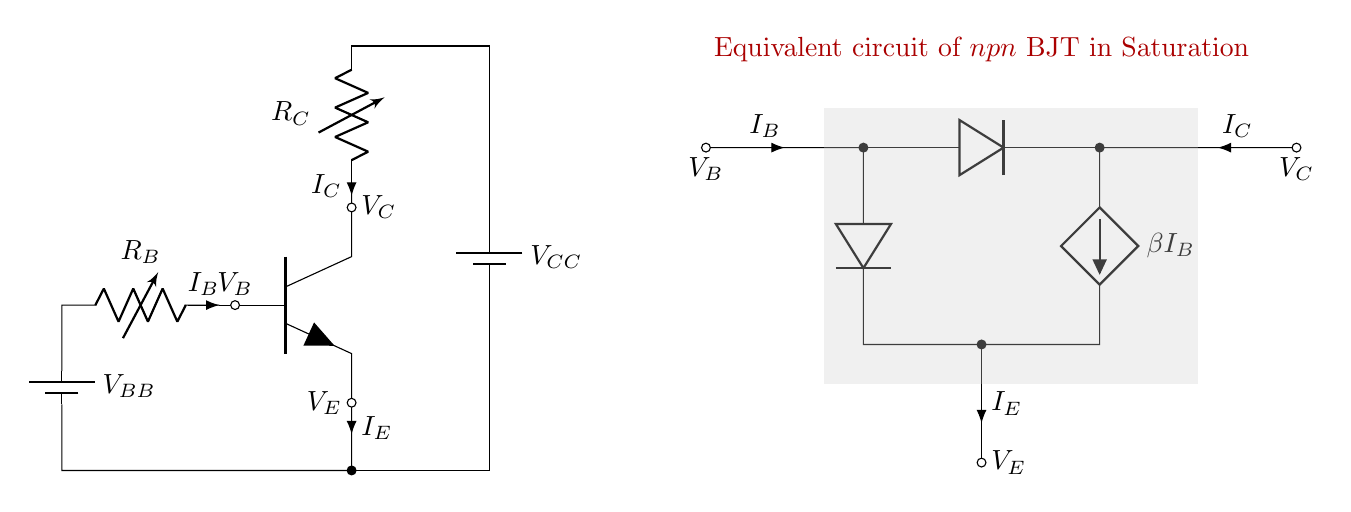
\begin{tikzpicture}
    \begin{scope}
        % npn BJT sumbol
        \draw (0, 0) node[npn, scale=2.0] (Q) {};
        \draw (Q.base) 
            to[vR, l_=$R_B$, invert, mirror] ++(-2.0, 0)
            to[battery1, l=$V_{BB}$] ++(0, -2.1)
            to ++(3.68, 0) node[circ] () {}
            to (Q.emitter);
        \draw (Q.collector)
            to[vR, l=$R_C$, mirror] ++(0, 1.75)
            to ++(1.75, 0)
            to[battery1, l=$V_{CC}$] ++(0, -5.39)
            to ++(-1.75, 0);
        % Current arrows
        \draw[-Latex, thin] (Q.base) ++(-0.4, 0.0) -- ++(0.4, 0) node[above, midway] {$I_B$};
        \draw[Latex-, thin] (Q.emitter) ++(0.0, -0.1) -- ++(0, 0.15) node[midway, right] {$I_E$};
        \draw[-Latex, thin] (Q.collector) ++(0, 0.1) -- ++(0, -0.25) node[midway, left] {$I_C$};
        % Add the transistor nodes.
        \node[ocirc] at ($(Q.base) + (0.2, 0)$) {};
        \node[anchor=south] at ($(Q.base) + (0.2, 0)$) {$V_B$};
        \node[ocirc] at ($(Q.emitter) + (0, 0.3)$) {};
        \node[anchor=east] at ($(Q.emitter) + (0, 0.3)$) {$V_E$};
        \node[ocirc] at ($(Q.collector) + (0, -0.3)$) {};
        \node[anchor=west] at ($(Q.collector) + (0, -0.3)$) {$V_C$};
    \end{scope}
    \begin{scope}[xshift=4.5cm, yshift=2.0cm]
        \node[anchor=center, color=myred] at (3.5, 1.25) {Equivalent circuit of $npn$ BJT in Saturation};
        % npn BJT sumbol
        \draw (0, 0) node[ocirc, anchor=center] (B) {}
            to ++(2, 0) 
            to[diode] ++(0, -2.5)
            to ++(3, 0)
            to[cI, l_={$\beta I_{B}$}, invert] ++(0, 2.5)
            to ++(2.5, 0) node[ocirc] (C) {};
        \draw (2, 0) node[circ] () {}
            to[diode] ++(3, 0) node[circ] () {};
        \draw (3.5, -2.5) node[circ] () {}
            to ++(0, -1.5) node[ocirc] (E) {};
        \node[anchor=north] at (B) {$V_B$};
        \node[anchor=north] at (C) {$V_C$};
        \node[anchor=west] at (E) {$V_E$};
        % Currents
        \draw[-Latex, thin] (B) ++(0.5, 0.0) -- ++(0.5, 0) node[above, midway] {$I_B$};
        \draw[-Latex, thin] (C) ++(-0.5, 0.0) -- ++(-0.5, 0) node[above, midway] {$I_C$};
        \draw[-Latex, thin] (E) ++(0, 1.0) -- ++(0,- 0.5) node[right, midway] {$I_E$};
        % Transparent filled dashed rectangle
        \fill[gray!40, opacity=0.3] 
            ($(B) + (1.5, 0.5)$) 
            rectangle ++(4.75, -3.5);
    \end{scope}
\end{tikzpicture}
\end{document}